\section{EXPERIMENTS}
\label{sec:experiment}

\begin{table*}
\caption{Test time 0.97-Timeliness measurement of different methods on \Grain. We break
 the methods into OMP, FR and Oracle family: e.g., ``Single" in the G-CS-OMP family means G-CS-OMP-Single, and ``FR" in the Oracle family means the oracle curve derived from G-FR. }
\label{tab:grain_auc} 
\begin{center}
\resizebox{0.7\textwidth}{!}{
\begin{tabular}{cccc|c|cc|c}
\multicolumn{4}{c|}{CS-G-OMP-Variants} &
\multicolumn{1}{c|}{CS-G-FR} &
\multicolumn{2}{c|}{Oracles} &
\multicolumn{1}{c}{Sparse} \\
	CS-G-OMP & 
	Single & 
	No-Whiten & 
	G-OMP & 
	\; & 
	FR Oracle &
	OMP Oracle &
  \; \\
  \hline
	\textbf{0.4406} & %G-OMP & 
	0.4086 &%G-OMP-Single & 
	0.4340 &%G-OMP-No-Whiten & 
	0.4073 &%G-OMP-Ignore-Cost & 
	\textbf{0.4525} &%G-FR 		& 
	\textbf{0.4551} & %FR Oracle \\
	0.4508 & % OMP oracle
  0.3997 \\
\end{tabular}
}
\end{center}
\end{table*}

\begin{table*}
\caption{Test time 0.99-Timeliness measurement of different methods on \YahooLTR.}
\label{tab:yahoo_auc} 
\begin{center}
\resizebox{0.7\textwidth}{!}{
\begin{tabular}{c|cccc|c|cc|c}
Group &
\multicolumn{4}{c|}{CS-G-OMP-Variants} &
\multicolumn{1}{c|}{CS-G-FR} &
\multicolumn{2}{c|}{Oracles} &
\multicolumn{1}{c}{Sparse} \\
	Size &
	CS-G-OMP & 
	Single & 
	No-Whiten & 
	G-OMP & 
	\; & 
	FR &
	OMP &
  \; \\
\hline
	5      & %Group Size
	\textbf{0.3188} & %G-OMP & 
	0.3039 &%G-OMP-Single & 
	0.3111 &%G-OMP-No-Whiten & 
	0.2985 &%G-OMP-Ignore-Cost & 
	\textbf{0.3222} &%G-FR 		& 
	\textbf{0.3225} & % FR oracle
	0.3211 & %Oracle \\  
  0.2934 \\

	10      & %Group Size
	\textbf{0.3142} & %G-OMP & 
	0.3117 &%G-OMP-Single & 
	0.3079 &%G-OMP-No-Whiten & 
	0.2909 &%G-OMP-Ignore-Cost & 
	\textbf{0.3205} &%G-FR 		& 
	\textbf{0.3207} & % FR oracle
	0.3164 & %Oracle \\  
  0.2858 \\

	15      & %Group Size
	\textbf{0.3165} & %G-OMP & 
	0.3159 &%G-OMP-Single & 
	0.3116 &%G-OMP-No-Whiten & 
	0.2892 &%G-OMP-Ignore-Cost & 
	\textbf{0.3213} &%G-FR 		& 
	\textbf{0.3213} & % FR oracle
	0.3177 & %Oracle \\  
  0.2952 \\

	20     & %Group Size
	\textbf{0.3161} & %G-OMP & 
	0.3124 &%G-OMP-Single & 
	0.3065 &%G-OMP-No-Whiten & 
	0.2875 &%G-OMP-Ignore-Cost & 
	\textbf{0.3180} &%G-FR 		& 
	\textbf{0.3180} & % FR oracle
	0.3163 & %Oracle \\ 
  0.2895 \\

\end{tabular}
}
\end{center}
\end{table*}


\begin{figure}
\centering
\subfloat[Training Time OMP vs. FR (\Grain)]{
  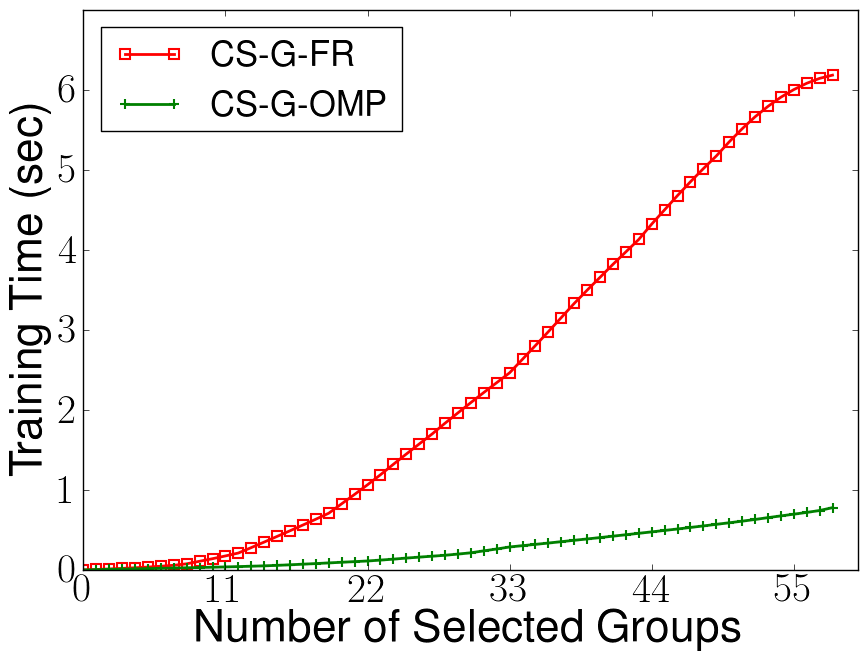
\includegraphics[width=0.37\textwidth,height=3.5cm]{\GOMPDIR/img/set1_exp4.png}
}

\subfloat[Training Time OMP vs. FR (\YahooLTR)]{
  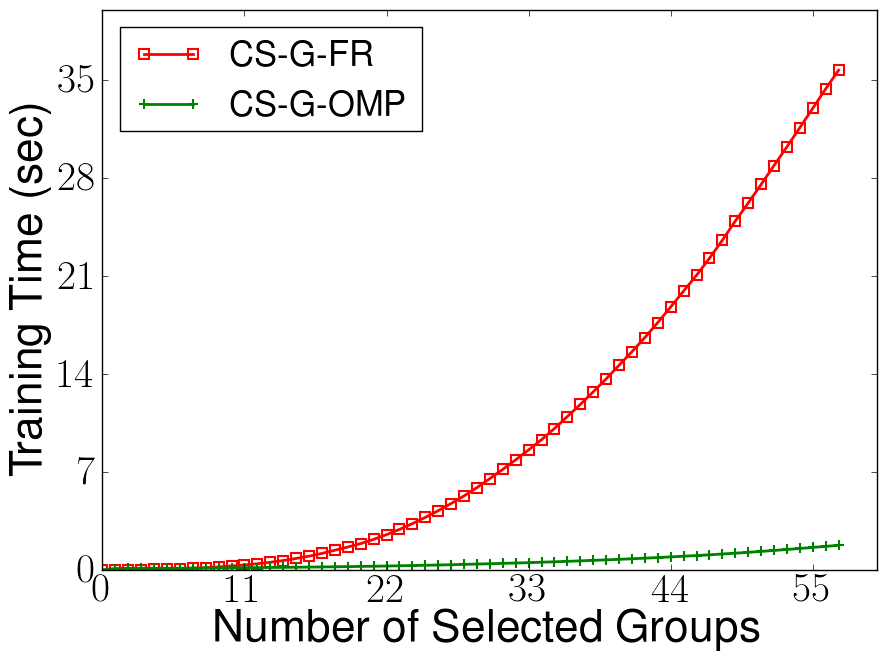
\includegraphics[width=0.37\textwidth,height=3.5cm]{\GOMPDIR/img/set1_size10_exp4.png}
}
\caption{The training time vs. the number of feature groups selected with two algorithms: CS-G-FR and 
CS-G-OMP. CS-G-OMP achieves a 8x and 20x overall training time speed-up 
on \Grain\, and \YahooLTR.} 
\label{fig:run_time}
\end{figure}

\subsection{DATA-SETS AND SET-UP}
We experiment our methods for anytime linear prediction on two real-world data-sets,
each of which has a significant number of feature groups with associated costs. 

\begin{itemize}[leftmargin=*]
\item \textbf{Yahoo! Learning to Rank Challenge} \citep{yahoo_ltr}
contains 883k web documents, each of which has a relevance score in $\{0, 1, 2, 3, 4\}$. Each of the 501 document features has an associated computational cost in 
$\{ 1, 5, 20, 50, 100, 150, 200\}$; the total feature cost is around 17K. The original data-set has no feature group structures, so we generated random group structures by grouping features of the same cost into groups of a given size $s$.\footnote{We experiment on group sizes $s \in \{ 5, 10, 15, 20 \}$. We choose regularizer 
$\lambda = 10^{-5}$ based on validation. We use 
$s=10$ for qualitative results such as plots and illustrations, but we report quantitative results for all group size $s$. For our quantitative results, we report the average test performance. The initial risk is $R(\emptyset)=0.85$.}

\item \textbf{Agriculture} is a proprietary data-set that contains 510k data samples, 328 features, and 57 feature groups. Each sample has a binary label in $\{1, 2\}$. Each feature group has an associated cost measured in its 
average computation time.\footnote{
There are 6 groups of size 32; the other groups have sizes between 1 and 6. 
The cost of each group is its expected computation time in seconds, ranging between 0.0005 and 0.0088; the total feature cost is 0.111. 
We choose regularizer $\lambda = 10^{-7}$. The data-set is 
split into five 100k sets, and the remaining 10k are used for validation. We report the cross validation results on the five 100K sets as the test results. The initial risk is $R(\emptyset) = 0.091$.}
\end{itemize}

\subsection{EVALUATION METRIC, BASELINE AND ORACLE}
\label{sec:timeliness}
\begin{figure}[t]
\centering
\subfloat[Plateau Effect and $\alpha$-Stopping Costs]{
 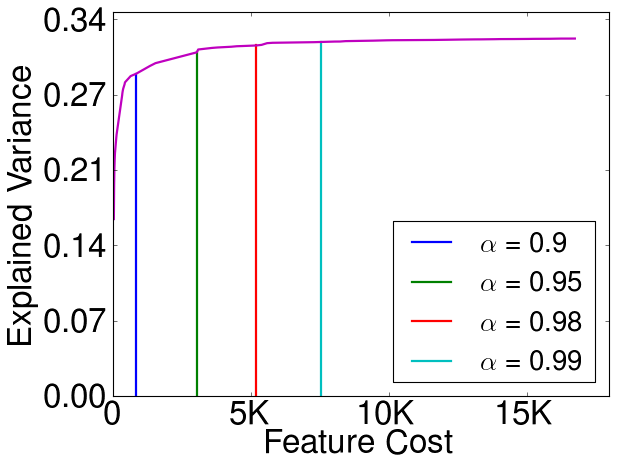
\includegraphics[width=0.40\textwidth,height=3.8cm]{\GOMPDIR/img/timeliness.png}
 \label{fig:timeliness_a}
}

\subfloat[Importance of Costs (CS-G-OMP vs. G-OMP)]{
 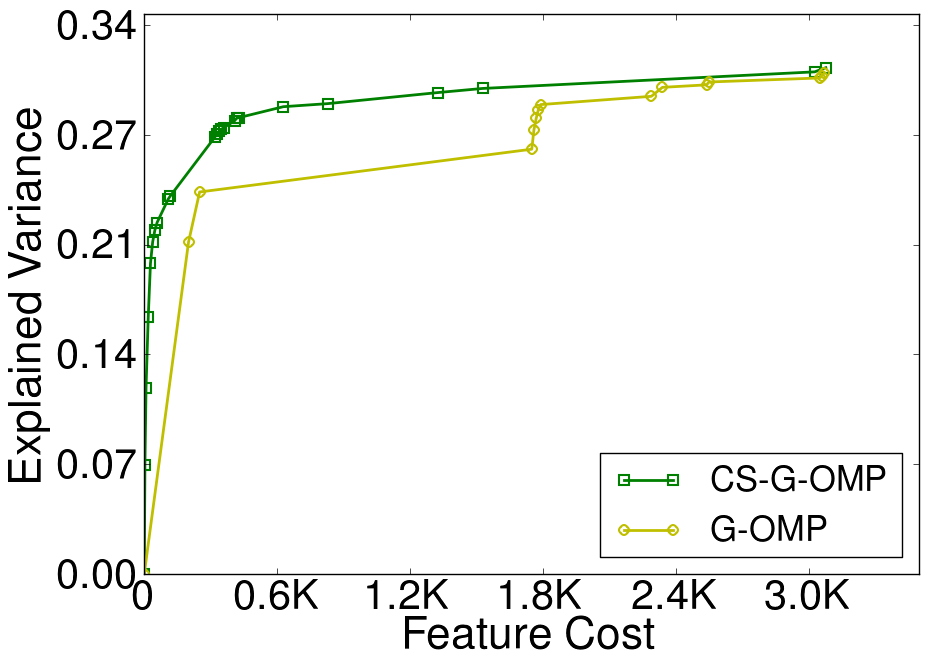
\includegraphics[width=0.40\textwidth,height=3.8cm]{\GOMPDIR/img/set1_size10_exp2.png}
 \label{fig:cost_vs_no_cost}
}
\label{fig:timeliness}
\caption{(a) Explained Variance vs. Cost curve of CS-G-OMP in
\YahooLTR. Vertical lines mark different $\alpha$-stopping costs.  (b) Explained Variance vs. Cost curve of CS-G-OMP and G-OMP on \YahooLTR\, set 1 with individual group size $s=10$, stopped at 0.97-stop cost.}
\end{figure}

Following the practice of \cite{timeliness}, we use the area under the 
maximization objective $F$ (explained variance) vs. cost curve normalized by the total area as the 
\textit{timeliness} measurement of the anytime performance of an algorithm\footnotetext{\cite{timeliness} define \textit{timeliness} as the area under the average precision vs. time curve}. In our data-sets, the performance of linear predictors plateaus much before
all features are used, e.g., Figure~\ref{fig:timeliness_a} demonstrates this effect in \YahooLTR, where the last one percent of total improvement is bought by half of the total feature cost. Hence the majority of the timeliness measurement is from the plateau performance of linear predictors. The difference between timeliness of different anytime algorithms diminishes due to the plateau effect. Furthermore, the difference vanishes as we include additional redundant high cost features. To account for this effect, we 
stop the curve when it reaches the plateau.
We define an \textit{$\alpha$-stopping cost} for parameter $\alpha$ in $[0,1]$ as the cost at which our CS-G-OMP achieves $\alpha$ of the final objective value in training and ignore the objective vs. cost curve after
the $\alpha$-stopping cost. We call the timeliness measure on the shortened curve 
as \textit{$\alpha$-timeliness}; 1-timeliness equals the normalized area under the full curve and 0-timeliness is zero. If a curve does not pick a group at $\alpha$-stopping cost, we linearly interpolate the objective value at the stopping cost to 
computr timeliness. 
We say an objective vs. cost curve has reached its final plateau if at least 95\% of the total 
objective has been achieved and the next 1\% requires more than 20\%
feature costs. (If the plateau does not exist, we use $\alpha = 1$.) Following this rule, we choose $\alpha = 0.97$ for \Grain\ and $\alpha = 0.99$ for \YahooLTR.

Since an exhaustive search for the best feature sequencing is intractable, 
we approximate with the \textbf{Oracle} anytime performance following the approach of \cite{timeliness}. Given an objective vs. cost curve of a sequencing, we reorder the feature groups in descending order of their marginal benefit per unit cost, assuming that the marginal benefits stay the same after reordering. We specify which sequencing is used for creating \textbf{Oracle} in Section~\ref{sec:selection_methods}. 
For baseline performance, we use cost-weighted Group Lasso \citep{group_lasso}, which
scales the regularization constant of each group with the cost of the group. We note that the cascade design by 
\cite{chen:12} can be reduced to this baseline if we enforce
linear prediction. 
More specifically, the baseline solves the following minimization problem:
\mbox{$
  \min _{w \in \mathbb{R}^{D}} \Vert Y -
    Xw \Vert^2_2 + \lambda
    \sum _{j=1}^J c(\mathcal{G}_j) \Vert w _{\mathcal{G}_j} \Vert _2,
$}
and we vary value of regularization constant
$\lambda$ to obtain lasso paths. We call this baseline algorithm \textbf{Sparse}\footnote{We use an off-the-shelf software, 
SPAMS (SPArse Modeling Software \citep{spams}), to solve the optimization.}.


\subsection{FEATURE COST}
Our proposed CS-G-OMP differs from Group Orthogonal Matching Pursuit (G-OMP) \citep{gomp} in that G-OMP does not consider feature costs when evaluating features. We show that this difference is crucial for anytime linear prediction. In Figure~\ref{fig:cost_vs_no_cost}, we compare the objective vs. costs curves of CS-G-OMP and G-OMP that are stopped at 0.97-stopping cost on \YahooLTR. As expected, CS-G-OMP achieves a
better overall prediction at every budget, qualitatively demonstrating the importance of incorporating feature costs. Table~\ref{tab:grain_auc} and Table~\ref{tab:yahoo_auc} 
quantify this effect, showing that CS-G-OMP 
achieves a better timeliness
measure than regular G-OMP. 

\subsection{GROUP WHITENING}
%Compare different normalization methods: whiten the whole data, 
%zero mean normalize, whiten each group. \and 
We provide experimental evidence that  
Group whitening, i.e., $X_g^TX_g = I_{D_g}$ for each group $g$, is a key assumption of both this work and previous feature group selection literature  by \cite{gomp, log_gomp}.
In Figure~\ref{fig:whiten_vs_no_whiten}, we compare 
anytime prediction performances using group whitened data 
against those using the common  
normalization scheme where each feature dimension
is individually normalized to have zero mean and unit variance. 
The objective vs. cost curve qualitatively shows that group whitening consistently results in the better predictions.
This behavior is expected from data-sets whose feature groups contain correlated features, e.g., group whitening effectively prevents selection step $(*)$ from overestimating the predictive power of feature groups of repeated good features. Table~\ref{tab:grain_auc} and Table~\ref{tab:yahoo_auc} demonstrate quantitatively the consistent better timeliness performance of CS-G-OMP over that of CS-G-OMP-no-whiten. 


\begin{figure}
\centering
\subfloat[Group Whiten vs. No-Whiten (\Grain)]{
  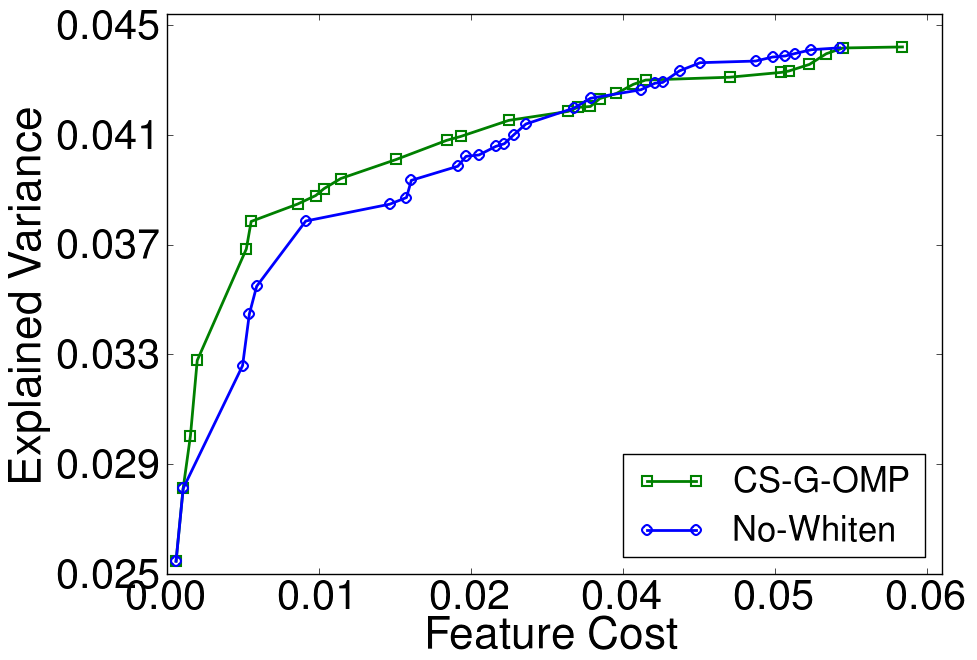
\includegraphics[width=0.4\textwidth,height=3.8cm]{\GOMPDIR/img/set1_exp1.png}
}

\subfloat[Group Whiten vs. No-Whiten (\YahooLTR)]{
  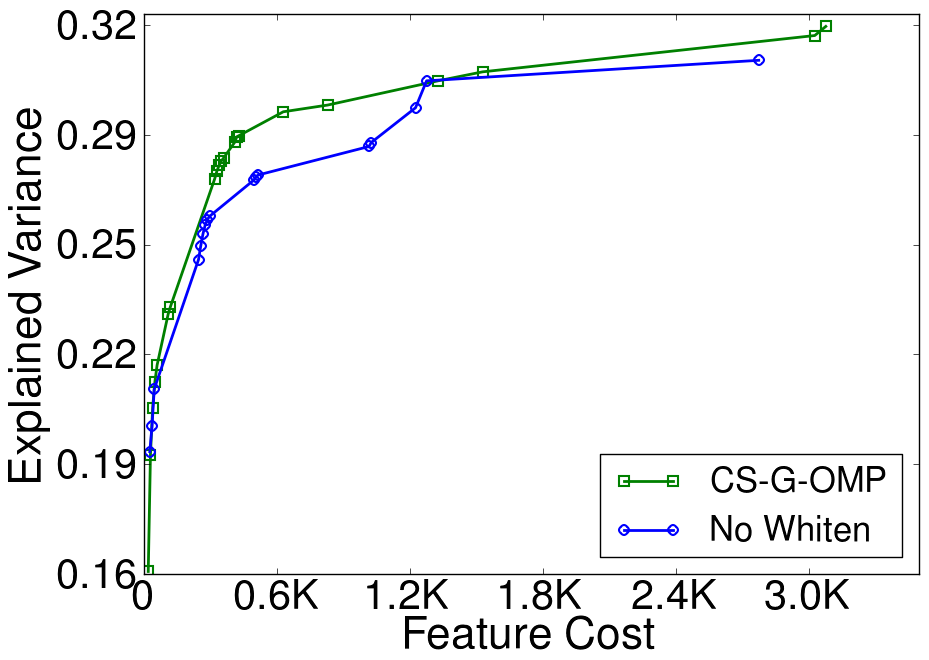
\includegraphics[width=0.4\textwidth,height=3.8cm]{\GOMPDIR/img/set1_size10_exp1.png}
}
\caption{Explained Variance vs. Feature Cost curves on \Grain\, (a) and \YahooLTR\, (b)  comparing group whitening with no group whitening. The curves stop at 0.97-stopping cost.}
\label{fig:whiten_vs_no_whiten}
\end{figure}


\subsection{SELECTION CRITERION VARIANTS}
\label{sec:selection_methods}
%FR vs OMP; group vs single

This section compares CS-G-OMP and CS-G-FR, along with 
variants of these two methods and the baseline, Sparse. 
We formulated the variant of CS-G-OMP, \textit{single}, in Section~\ref{sec:method} and it intuitively chooses feature groups of the best single feature dimension per group cost. Our experiments show that this modification degrades prediction performance of CS-G-OMP. 
%If we enforce linear prediction, cascade design by \cite{cai:15} can be reduced to a greedy method whose criteria is the G-OMP criteria subtracted by a function of the feature cost. However, this method requires careful tuning of the 
Since FR directly optimizes the objective at each step, we expect CS-G-FR to perform the best and use its curve to compute the \textbf{Oracle} curve as an approximate to the best achievable performance.

In Figure~\ref{fig:selection_methods}, we evaluate CS-G-FR, CS-G-OMP and CS-G-OMP-single based on the objective in Theorem~\ref{thm:main}, i.e., explained variance vs. feature cost curves. 
CS-G-FR, as expected, outperforms all other methods. CS-G-OMP outperforms the baseline method, Sparse, and the CS-G-OMP-Single variant. 
The performance advantage of CS-G-OMP over CS-G-OMP-Single is much clearer in the \Grain\ data-set than in the \YahooLTR\ data-set. \Grain\ has a natural group structure which may contain correlated features in each group. \YahooLTR\ has a randomly generated group structure whose features were filtered by feature selection before the data-set was published \citep{yahoo_ltr}. CS-G-FR and CS-G-OMP outperform the baseline algorithm, Sparse. We speculate that linearly scaling group regularization constants by group costs did not enforce Group-Lasso to choose the most cost-efficient features early. 
The test-time timeliness measures of each of the methods are recorded in Table~\ref{tab:grain_auc} and Table~\ref{tab:yahoo_auc},
and quantitatively confirm the analysis above. Since \Grain\, and \YahooLTR\, are originally a classification and a ranking data-set, respectively, we also report in Figure~\ref{fig:selection_methods} the performance using classification accuracy and NDCG@5. This demonstrates the same qualitatively results as using explained variants. 

%We note that on the two real-world data-sets, Doubling Algorithm acts identically to CS-G-FR after few initial selections, an expected result because real-world feature effectiveness does not grow exponentially in cost, so that the most cost-efficient features become available to Doubling after few steps. 


\begin{figure}
\centering
\subfloat[FR vs. OMP vs. Sparse (\Grain)]{
  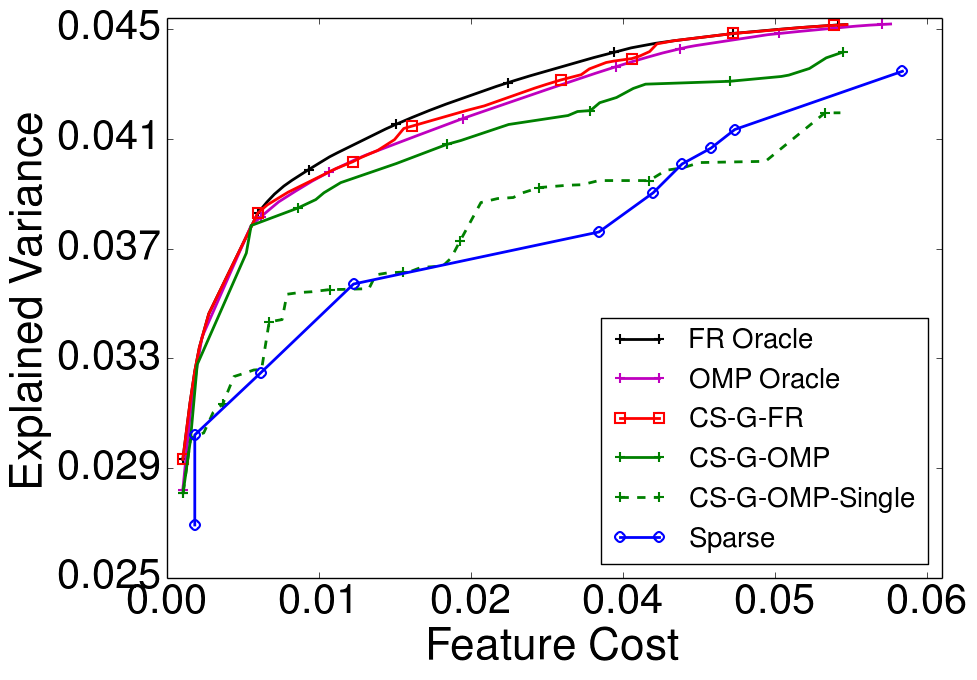
\includegraphics[width=0.40\textwidth,height=4cm]{\GOMPDIR/img/set1_exp3.png}
}

\subfloat[FR vs. OMP vs. Sparse (\YahooLTR)]{
  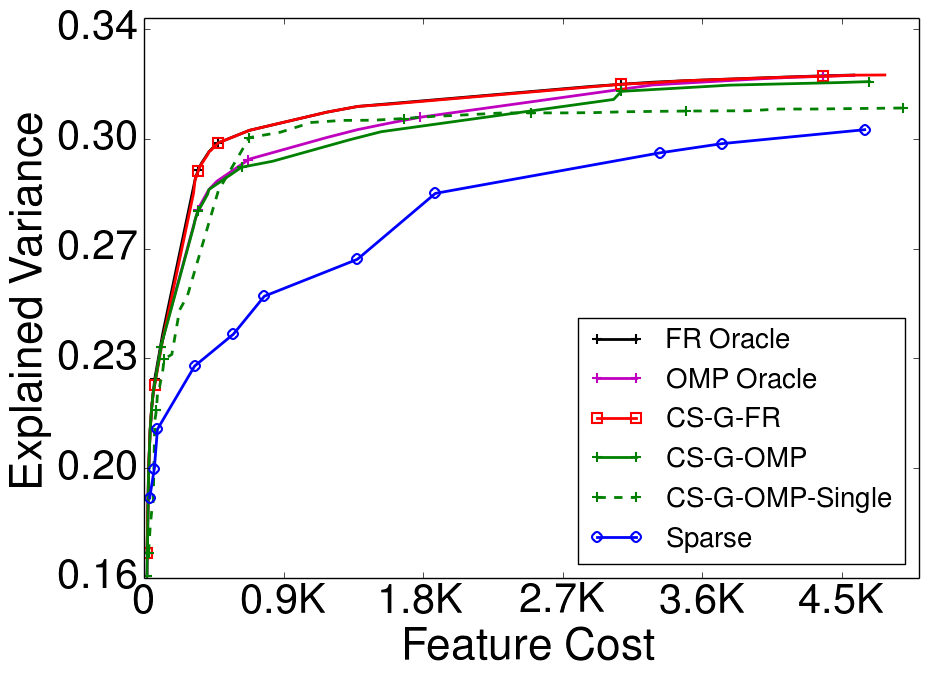
\includegraphics[width=0.40\textwidth,height=4cm]{\GOMPDIR/img/set1_size10_exp3.png}
}

\subfloat[FR vs. OMP vs. Sparse (\Grain)]{
  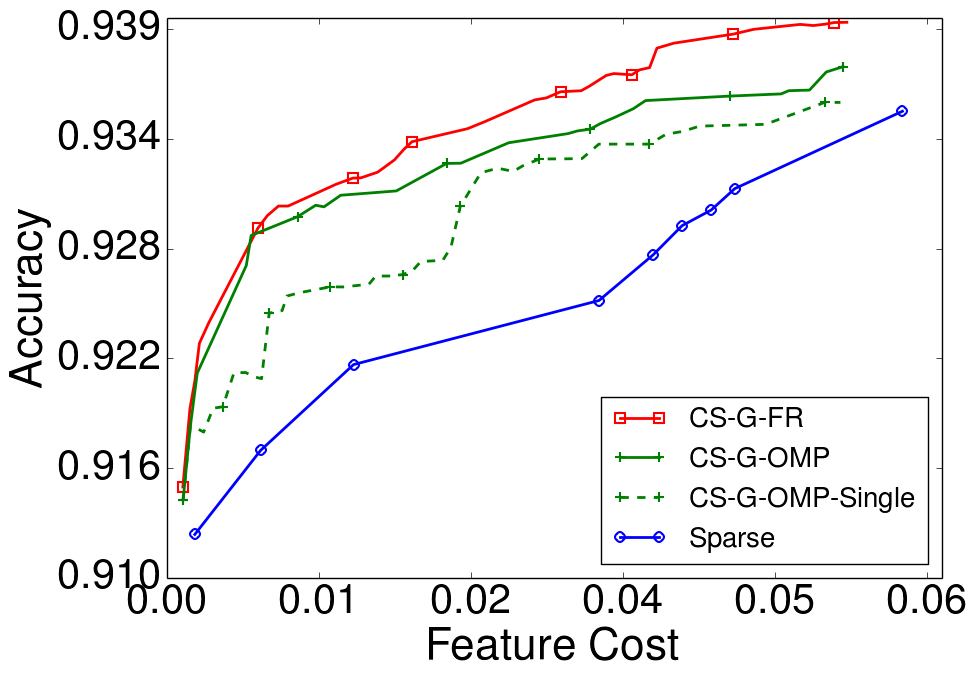
\includegraphics[width=0.40\textwidth,height=4cm]{\GOMPDIR/img/set1_exp5.png}
}

\subfloat[FR vs. OMP vs. Sparse (\YahooLTR)]{
  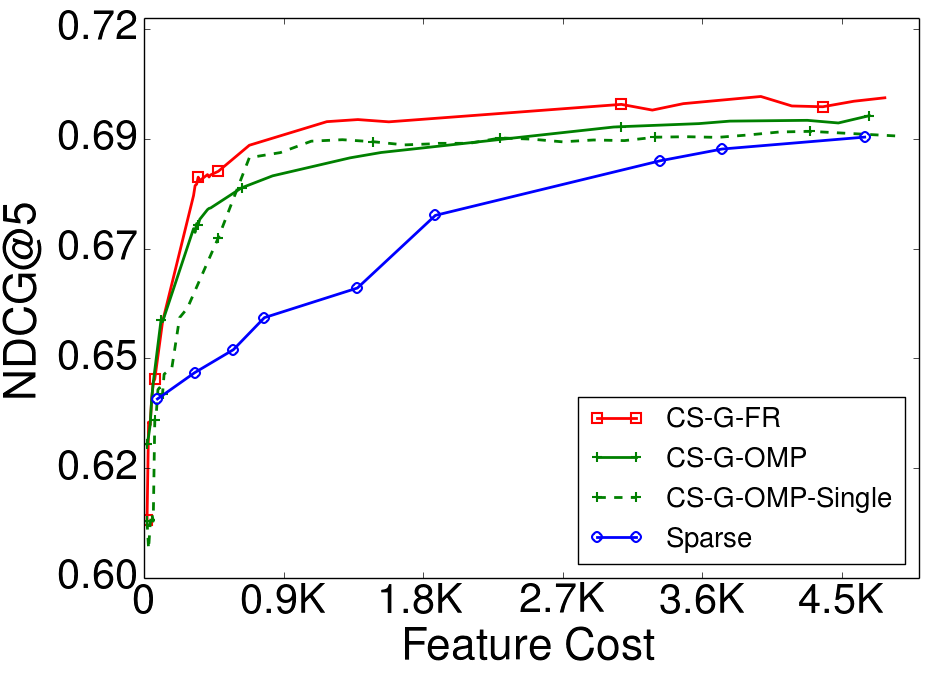
\includegraphics[width=0.40\textwidth,height=4cm]{\GOMPDIR/img/set1_size10_exp5.png}
}

\caption{(a),(b): Explained Variance vs. Feature Cost curves on 
\Grain\, and \YahooLTR (group-size=10), 
using CS-G-OMP, CS-G-FR and their Single variants. Curves stop at 0.97 and 0.98 stopping costs. (c),(d): Same curve with the natural objectives of the data-sets: accuracy and NDCG@5.} 
\label{fig:selection_methods}
\end{figure}

As expected, when compared against CS-G-OMP, CS-G-FR consistently chooses more cost-efficient features at the cost of a longer training time.
In the context of linear regression, let us assume that the group sizes are 
bounded by a constant when we are to select the number 
$K$ feature group. We can then compute a new model of $K$  groups in $O(K^2N)$ using
Woodbury's matrix inversion lemma, evaluate it in $O(KN)$, and compute the gradients with respect to the weights of unselected groups in $O(N(J-K))$. Thus, CS-G-OMP requires $O(K^2N + JN)$ at step $K=1,2,3,..., J$ and CS-G-FR requires $O((J-K)K^2N)$, so the total training  complexities for CS-G-OMP and CS-G-FR are $O(J^3N)$ and $O(J^4N)$, using $\sum_{K=1}^J K^2 = \frac{1}{6}J(J+1)(2J+1)$ and $\sum _{K=1}^J K^3 = \frac{1}{4}J^2(J+1)^2$. 
We also show this training complexity gap empirically in Figure~\ref{fig:run_time}, which plots the curves of training time vs. number of feature groups selected. When all feature groups are selected, CS-G-OMP achieves a 8x speed-up in \Grain\ over CS-G-FR. In \YahooLTR, CS-G-OMP achieves a speed-up factor between 10 and 20; the smaller the sizes of the groups, the larger speed-up due to the increase in the number of groups. Both greedy methods are much faster than the Lasso path computation using SPAMS, however. 


